% 
% Annual Cognitive Science Conference
% Sample LaTeX Paper -- Proceedings Format
% 

% Original : Ashwin Ram (ashwin@cc.gatech.edu)       04/01/1994
% Modified : Johanna Moore (jmoore@cs.pitt.edu)      03/17/1995
% Modified : David Noelle (noelle@ucsd.edu)          03/15/1996
% Modified : Pat Langley (langley@cs.stanford.edu)   01/26/1997
% Latex2e corrections by Ramin Charles Nakisa        01/28/1997 
% Modified : Tina Eliassi-Rad (eliassi@cs.wisc.edu)  01/31/1998
% Modified : Trisha Yannuzzi (trisha@ircs.upenn.edu) 12/28/1999 (in process)
% Modified : Mary Ellen Foster (M.E.Foster@ed.ac.uk) 12/11/2000
% Modified : Ken Forbus                              01/23/2004
% Modified : Eli M. Silk (esilk@pitt.edu)            05/24/2005
% Modified: Niels Taatgen (taatgen@cmu.edu)  10/24/2006

%% Change ``a4paper'' in the following line to ``letterpaper'' if you are
%% producing a letter-format document.

\documentclass[10pt,letterpaper]{article}

\usepackage{cogsci}
\usepackage{pslatex}
\usepackage{apacite}
\usepackage{graphicx}
\usepackage{color}


\title{ When does a near-miss sting? }
 
\author{{\large \bf Desmond C. Ong (dco@stanford.edu)} \\
{\large \bf Jamil Zaki (jzaki@stanford.edu)} \\
{\large \bf Noah D. Goodman (ngoodman@stanford.edu)} \\
  Department of Psychology, Stanford University, Stanford CA, USA 
}

%array of cards
%choose card
%winning card is either proximally closer or numerically closer

%proximally closer vs numerically closer vs different suit (diamond & heart vs. spade & club)
% 3 forced choice (A, B, or equal)

% die + card task

\begin{document}

\maketitle

\begin{abstract}
Near misses---missing the desired outcome by a small margin---are more emotionally intense than normal misses, even though the outcomes tend to be no different, and people readily accord near-miss effects when reasoning about others. Yet there are still open questions: what are the distance dimensions along which near misses are judged, and how do people incorporate near misses into more general affective cognition (or reasoning about emotion). In this paper we show that intuitive theories of emotion seem to weigh near-misses even for random events, and this is driven by the semblance of action-outcome contingency. Finally, we incorporate near misses into a larger model of affective cognition, and quantify the psychological cost of a near-miss relative to winning and losing.

\textbf{Keywords:} 
Near Miss; Counterfactual Distance; Lay Theories; Emotion
\end{abstract}


\begin{quote}
\textit{``Close only counts in horseshoes and hand grenades"} 
-- English Idiom
\end{quote}


	When Rob achieves a desired outcome, such as winning a soccer match, we intuitively know that he would feel positive. Conversely, when Rob fails to achieve an outcome, we can reason that he would feel negative. If he just fails to achieve the outcome by a small margin, a \textit{near-miss}, such as losing a soccer game by a single goal, we intuitively recognize that he actually would feel worse, because the outcome was so close. Penalty shootouts in soccer provides the most exaggerated of such near-miss scenarios: the losing team often loses because of one missed ball, sometimes an inch shy of escaping the goalkeeper's hands. These details add much more emotional intensity to all agents involved, more so than just a simple loss. Contrary to the above idiom, close counts---\textit{emotionally}.

	Such intuitive reasoning about emotions comprise what we call \textit{affective cognition}, or reasoning about emotions and other affective states (some citations xxx, Ong, Zaki, \& Goodman, under review). Psychologists have long known that near-misses form an integral, but surprisingly not well understood part of affective cognition \cite{Johnson1986, Gleicher1990}. Most of this work falls under the broader category of counterfactual thinking \cite{Bryne2002,McMullen2002, Medvec1997, Roese1997}. Near-miss counterfactuals are particularly engaging to think about, because these possible worlds almost happened: they were separated from the current world by some small ``distance". Consider \citeA{Kahneman1982}'s classic example of Mr Tees, who missed his plane by 5 minutes, and Mr Crane, who missed his plane by 30 minutes. Both men were delayed due to traffic, but people consistently and reliably judge the person who narrowly missed his plane to feel much worse than the one who missed it by a wider margin. One proposed \textit{causally-relevant} explanation for the near miss effect is that of controllability: Mr Tees could easily think of actions he could have done differently (``if only I woke up ten minutes earlier") that would have led to him catching the plane. 

	There however, remains many open questions, and we list just three of them here. First, what is the nature of these ``counterfactual distances" --- the distances that separate the desired-but-unattained counterfactual world from the current world. The answer most commonly proposed by the current literature asserts that people should consider causally-relevant dimensions, like the amount of time one misses a plane by. This would predict that people should not exhibit near miss effects in their lay theory when considering games of chance, or random events, as the causal process that generated the outcomes are based on chance. This however, is not intuitive; gamblers, for example, persist more after near misses, indicating a near-miss effect on motivation, even though the outcome of gambling tasks such as slots are independent of the gambler's actions \cite{Kassinove2001, Reid1986}. In Experiment 1, we show that observers readily judge an agent who ``narrowly misses" on a die game (by rolling a number close to the target number) to feel worse than one who misses by a larger amount, even though outcomes on a die game are not ordered like the number line.

Second, how do observers reason using these distance dimensions? Depending on the context, different dimensions of distance should matter to different extents. In Experiment 2, we show that observers are sensitive to contextual shifts that change the relevance of different distances in a random card-guessing task. 
\textcolor{red}{(to discuss with Noah more on this point. action-outcome contingency.)}

Finally, how much does a near-miss cost psychologically? That is, what is the relative size of near miss effects relative to actually winning or losing an amount. In Experiment 3, we build upon a previous model of affective cognition (Ong, Zaki, \& Goodman, under review) and explicitly incorporate modeling of near-miss effects into this quantitative model. This allows us to estimate relative effect sizes, and shed more light on their modeling.




%Spell out relevant and irrelevant. Deeper theory.

%Nearness compared to actual outcome differences



%Hmm maybe not the best example: even if the 7 mins was reduced to 0, they wouldn't necessarily have won.

%	Argentina nearly won the 2014 FIFA World Cup Final, conceding the only goal of the match with barely 7 minutes left in extra time, but as the above idiom morbidly points out\footnote{Points in horseshoes are scored based on distance thrown horseshoes land from the target stake. Thrown hand grenades, in contrast, do not need to hit their target to be effective.}, close in this case, does not count. However close they were, they did not win. However, as Argentinian supporters would attest, close does matter---\textit{emotionally}.



%	Though we live in only one of many possible realizations of the world, our mental lives---and consequently, our emotional lives---are constantly spent exploring other possible worlds via counterfactual thinking \cite{Bryne2002, Gleicher1990, Johnson1986, Roese1997}. ``Near-miss" or close counterfactual comparisons in particular, are so mentally engaging because these possible worlds had almost happened. Consider \citeA{Kahneman1982}'s classic example of missing a plane by 5 minutes, as opposed to 30 minutes: people consistently and reliably judge the person who narrowly missed his plane to feel much worse than the one who missed it by a wider margin. One proposed reason is that it is much easier to generate possible counterfactual antecedents that would have resulted in the counterfactual consequent of catching the plane. The near-miss character could easily generate counterfactuals like ``If only I woke up 5 minutes earlier" or ``if only I had packed my bag the night before", that would result in the consequent ``then I would have caught my plane". If the counterfactual world is somehow \textit{closer} to the current world, then perhaps the counterfactual world would only require a smaller change in the causal chain that led up to the current world in order to be realized.
%
%	Previous research has identified some of the impact of closeness on counterfactual thought \cite{Kahneman1990, Teigen1996}. Closeness increases the activation of counterfactual thought, by increasing the salience of the counterfactual world \cite{Kahneman1982, Roese1997}, and additionally also amplifies the affective consequence of the counterfactual comparison \cite{Johnson1986, Kahneman1982}. Narrowly missing a plane or a World Cup Title feels far worse than missing it by a large margin. 
%	
%	Yet, there remains many open questions regarding the nature of these distances. What are the relevant dimensions of closeness that people incorporate into their lay theories of the world, and into their lay theories of emotion? Intuitively, people should consider only causally-relevant dimensions, like the amount of time one misses a plane by. However, anecdotally we are reminded of many instances where a (randomly-generated) lucky draw number is announced, and the holder of a (randomly-assigned) lucky draw ticket that is off by 1 number expresses extreme negative emotions. Given the random nature of this game, his number is not any ``closer" to reality than any other number in the set of possibilities.
	
	

%\subsection{Outline of paper:}
%\begin{enumerate}
%\item Lay out near miss predictions. Noticably: clearly, on both win and lose sides.
%\item Expt 1: just show it with vignettes, where distance is causally related to outcome
%\item Expt 2: show it with die vignettes, where distance is irrelevant
%\item Expt 3: card task, show that the relevant dimension can be tweaked
%\end{enumerate}
%
%
%
%\subsection{Contributions:}
%\begin{enumerate}
%\item ToE takes into account near misses -- but along what dimensions?
%\item show robustly that it considers both neg and positive misses (expt1)
%\item show that it considers irrelevant distances
%\item 
%\end{enumerate}
%
%Any similarity, causal counterfactual
%control-relevant (exploitable) causal counterfactual
%covert utility differences



\textcolor{red}{(Only Experiment 2 is ready so far.).}

\section{Predictions}


\begin{figure}[htb!]
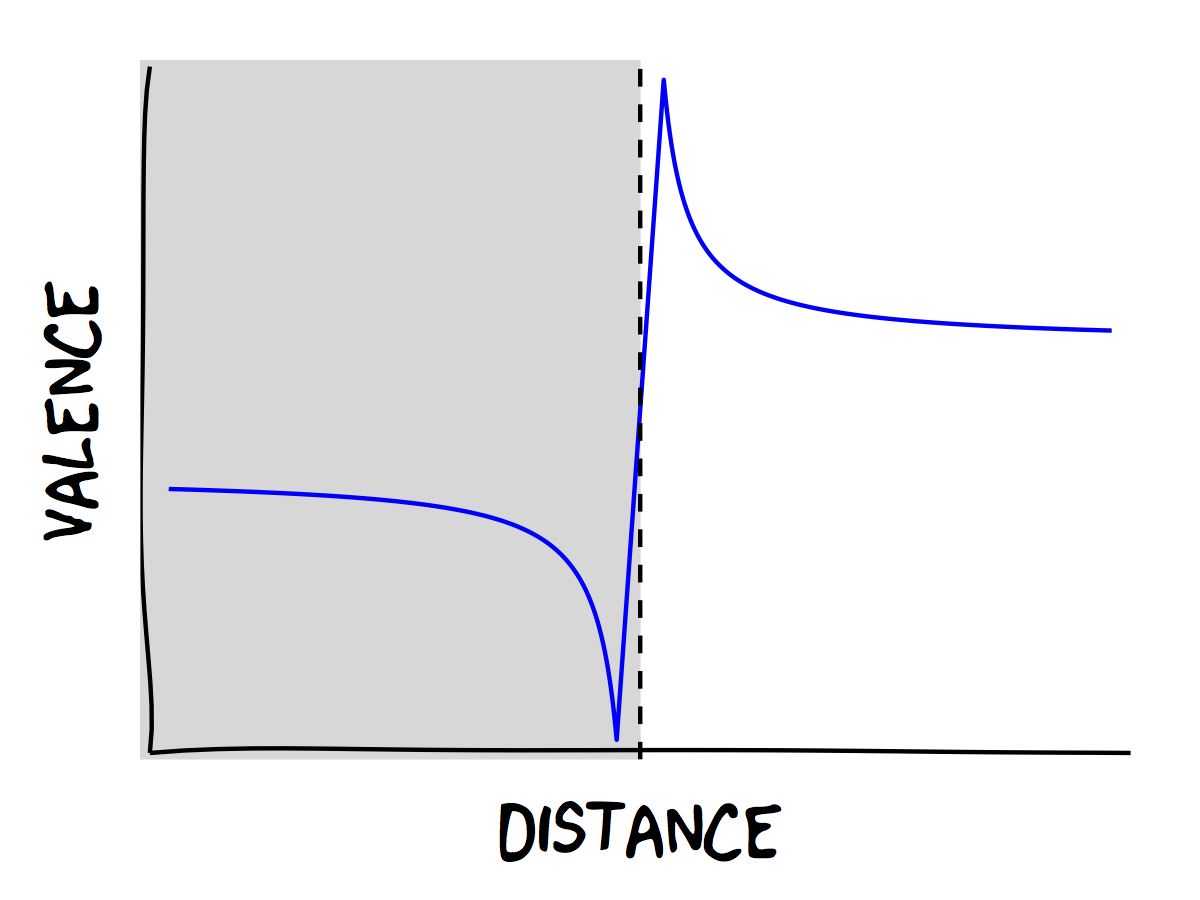
\includegraphics[width=\columnwidth]{images/predictionFig.png}
\caption{ Prediction.}
\label{PredictionFig}
\end{figure}

%
%\section{Experiment 1: Vignettes}
%In Experiment 1, participants made attributions of emotion to characters in ``near-miss" or ``just-hit" vignettes.
%
%\subsubsection{Materials.} We generated 6 vignettes that involved a dimension of ``distance" which was relevant to the outcome. There were two characters in each vignette. For example, in the ``freeGift" vignette, participants read about Scott and Frank who were both in line for a free brand new vacuum cleaner. Scott was 2nd in line when they ran out of free gifts, while Frank was number 10 when they ran out of free gifts. The possible distances shown were drawn from the following possible values: \{-50, -10, -2, 2, 10, 50\}, where negative values indicates not making the desired outcome. The example described above had distances of -10 and -2. The other vignettes involved: 2) just missing a plane, 3) getting tickets for a concert, 4) making it to a gelato shop before closing time, 5) getting admitted to a course at the local community college and 6) running out of paint when painting a fence.
%
%\subsubsection{Participants.} We recruited 100 participants through Amazon's Mechanical Turk and paid them for completing the experiment. All experiments reported in this paper were conducted according to guidelines approved by the Institutional Review Board at Stanford University.
%
%\subsubsection{Procedures.} Participants viewed each of the six vignettes in a random order. After each vignette, they answered several attention check questions, before rating how each character in the story felt, along six emotions: \{happiness, sadness, contentment, disappointment, relief, and regret\}. After they attributed emotions to both characters, participants made a forced choice rating: which character felt happier? They were also given a neutral option: ``Both feel equally happy".
%
%
%\begin{figure}[htb!]
%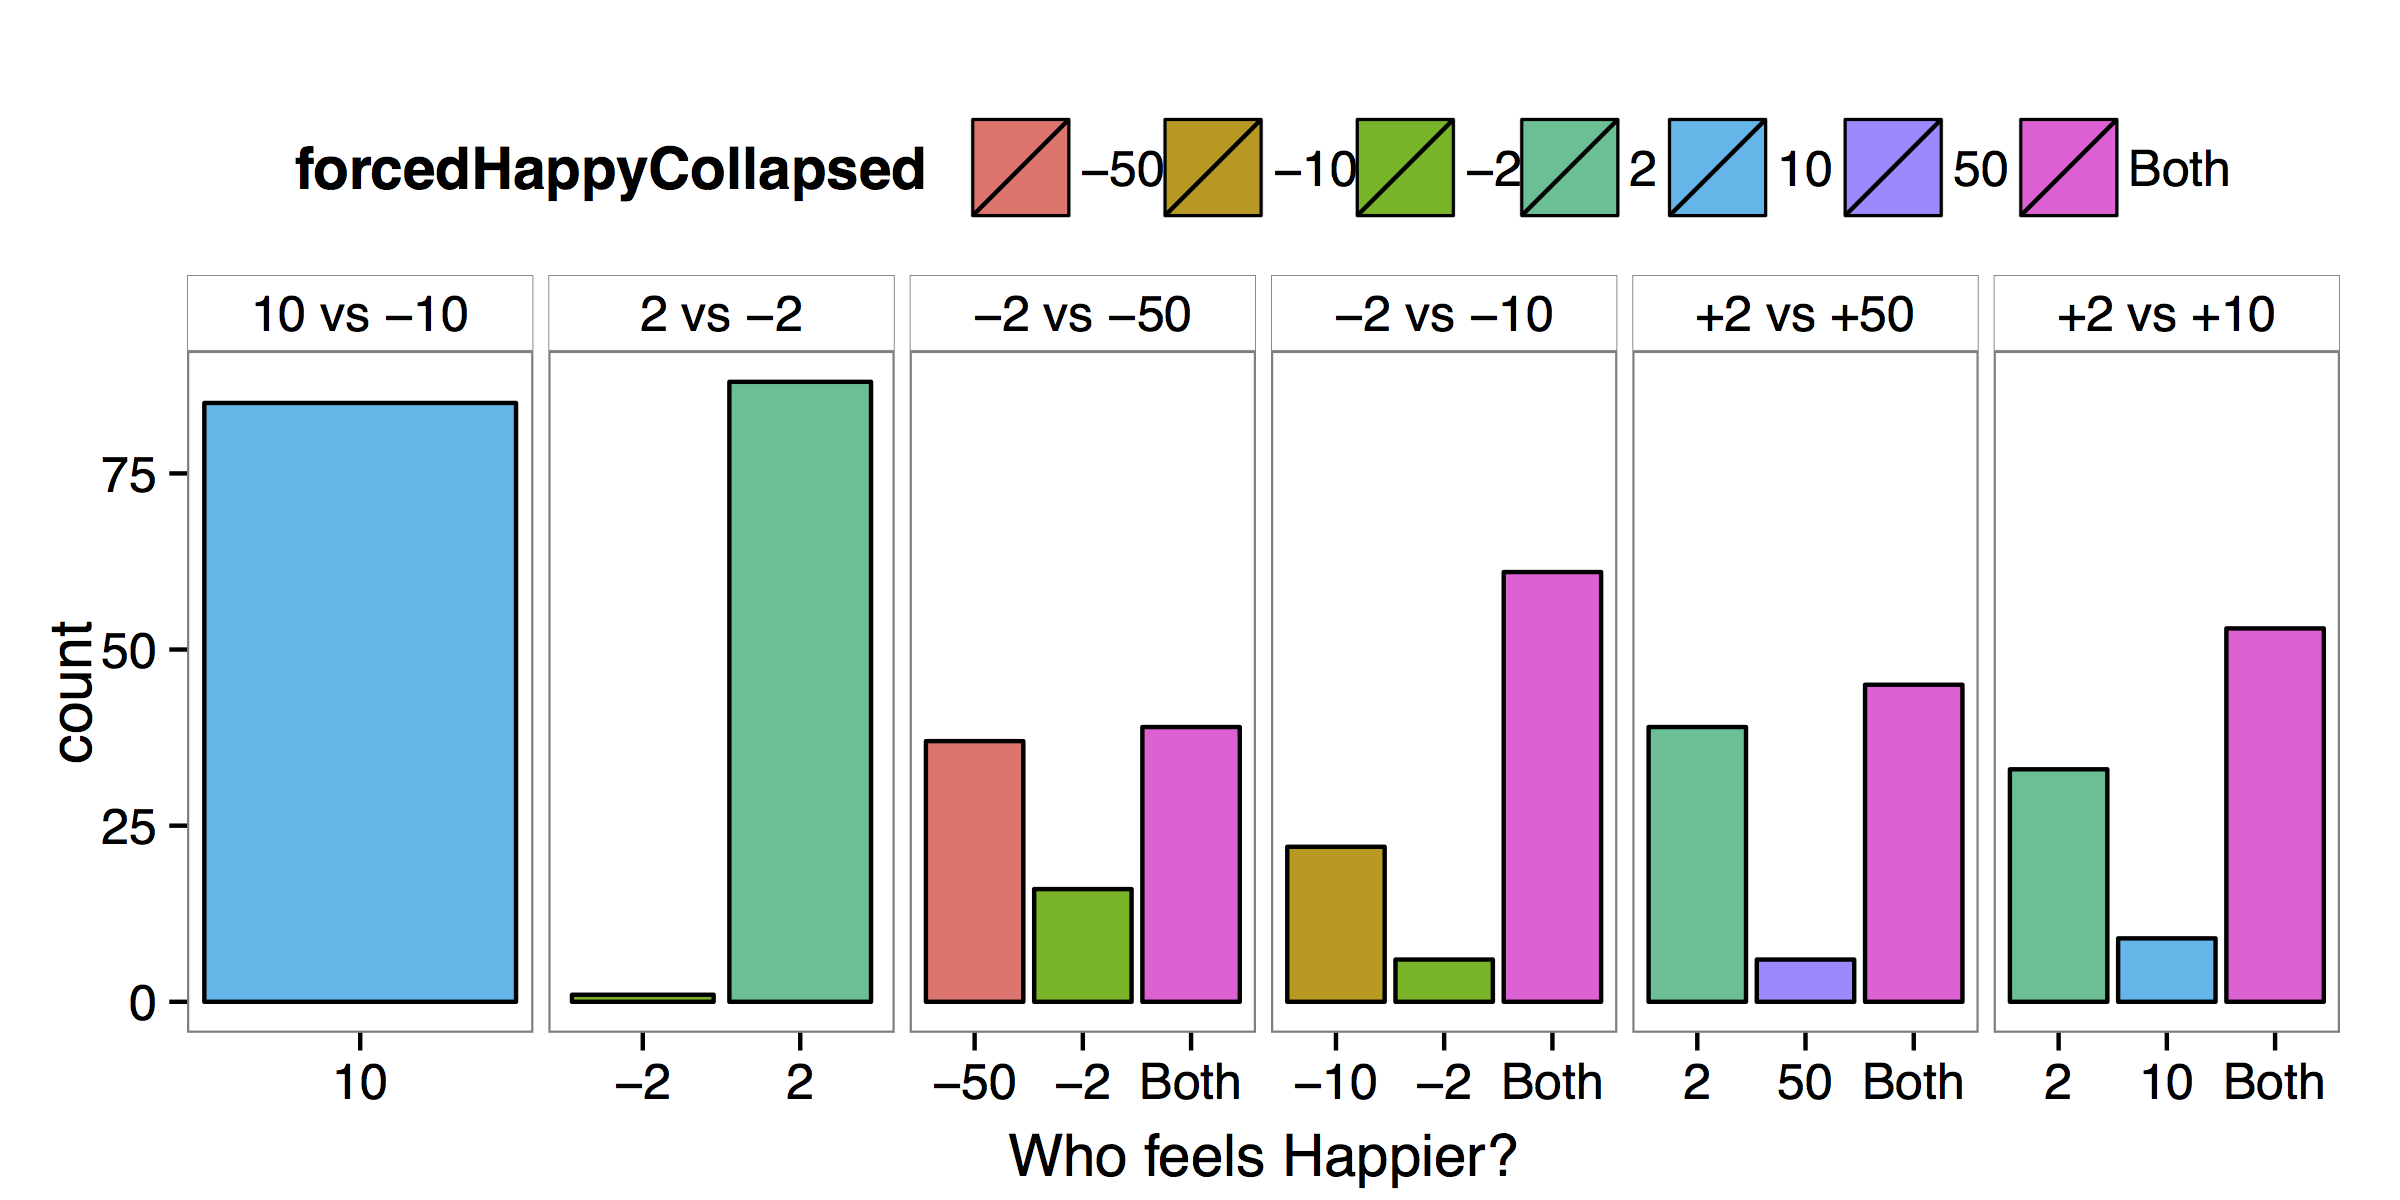
\includegraphics[width=\columnwidth]{images/vignettes_forcedHappy.png}
%\caption{ Expt 1 Results. Proportions of forced choice response to ``Who feels happier?". Error bars indicate standard errors. Answers are labeled with the distance of the character's outcome. E.g., in the right-most panel, more people judged the character who just made the outcome (+2) to be happier than the character who made it by a larger margin (+10).}
%\label{Expt1ResultFig}
%\end{figure}
%
%%%%% TODO XXX STATS
%
%\subsubsection{Results.} Post-hoc analysis showed that results were similar across five of the vignettes\footnote{The only anomaly was the fence painting vignette. In the critical comparison in that vignette, X ran out of paint with just 2 inches of fence left, while Y ran out with 10 inches left. Although we predicted that the near-miss character (X) would feel worse, painting a fence involves a persistent product rather than a once-off event: X could return to fence in the future, and he only needs to paint 2 more inches then. In this case, the more distance, the better. We excluded this vignette from the analyses.}: the character that experienced the near-miss (-2) was rated to feel worse than the character that experienced a further-miss (-10, -50) (TODO XXX STATS), and the character that just made the outcome (+2) was rated to feel better than the character that made the outcome by a large margin (+10, +50) (TODO XXX STATS).
%
%The forced choice results are given in Fig. \ref{Expt1ResultFig}. Across the win-lose comparison (left two panels), all participants rated the character who obtained the outcome to be happier. Across lose-lose comparisons, far fewer participants rated the near-miss character as feeling happier (TODO XXX STATS), and across win-win comparisons, far more participants rated the just-hit character as feeling happier (TODO XXX STATS). We note that a large proportion of participants chose the neutral option, and this proportion is higher than than the near-miss/just-hit judgments. 
%
%% 
%\textcolor{red}{\textit{COMMENT: do we interpret the high proportion of "Both" as meaning that it's a weak effect? or that there are individual differences, and majority of Ps might not be sensitive to this?}}
%
%

%\section{Experiment 1: Dice vignette}
%
%
%
%\begin{figure}[htb!]
%%\includegraphics[width=\columnwidth]{images/expt2results.png}
%\caption{ Expt 1 Results.}
%\label{Expt1ResultFig}
%\end{figure}


\section{Experiment 2: Changing the relevant dimensions}

We designed Experiment 2 to dissociate closeness effects along different dimensions. Using a card guessing task, we manipulated the task-relevance of both the positions of the cards or the numbers written on the cards, and showed that only near-miss effects along the task relevant-dimension are incorporated into observers' lay theory of emotion.

\subsubsection{Participants.} We recruited 300 participants through Amazon's Mechanical Turk, and assigned them to one of three conditions: Single-Trial-Position (N=100), Two-Trial-Position (N=100), Single-Trial-Number (N=100).


\subsubsection{Procedures.} 

\begin{figure}[htb!]
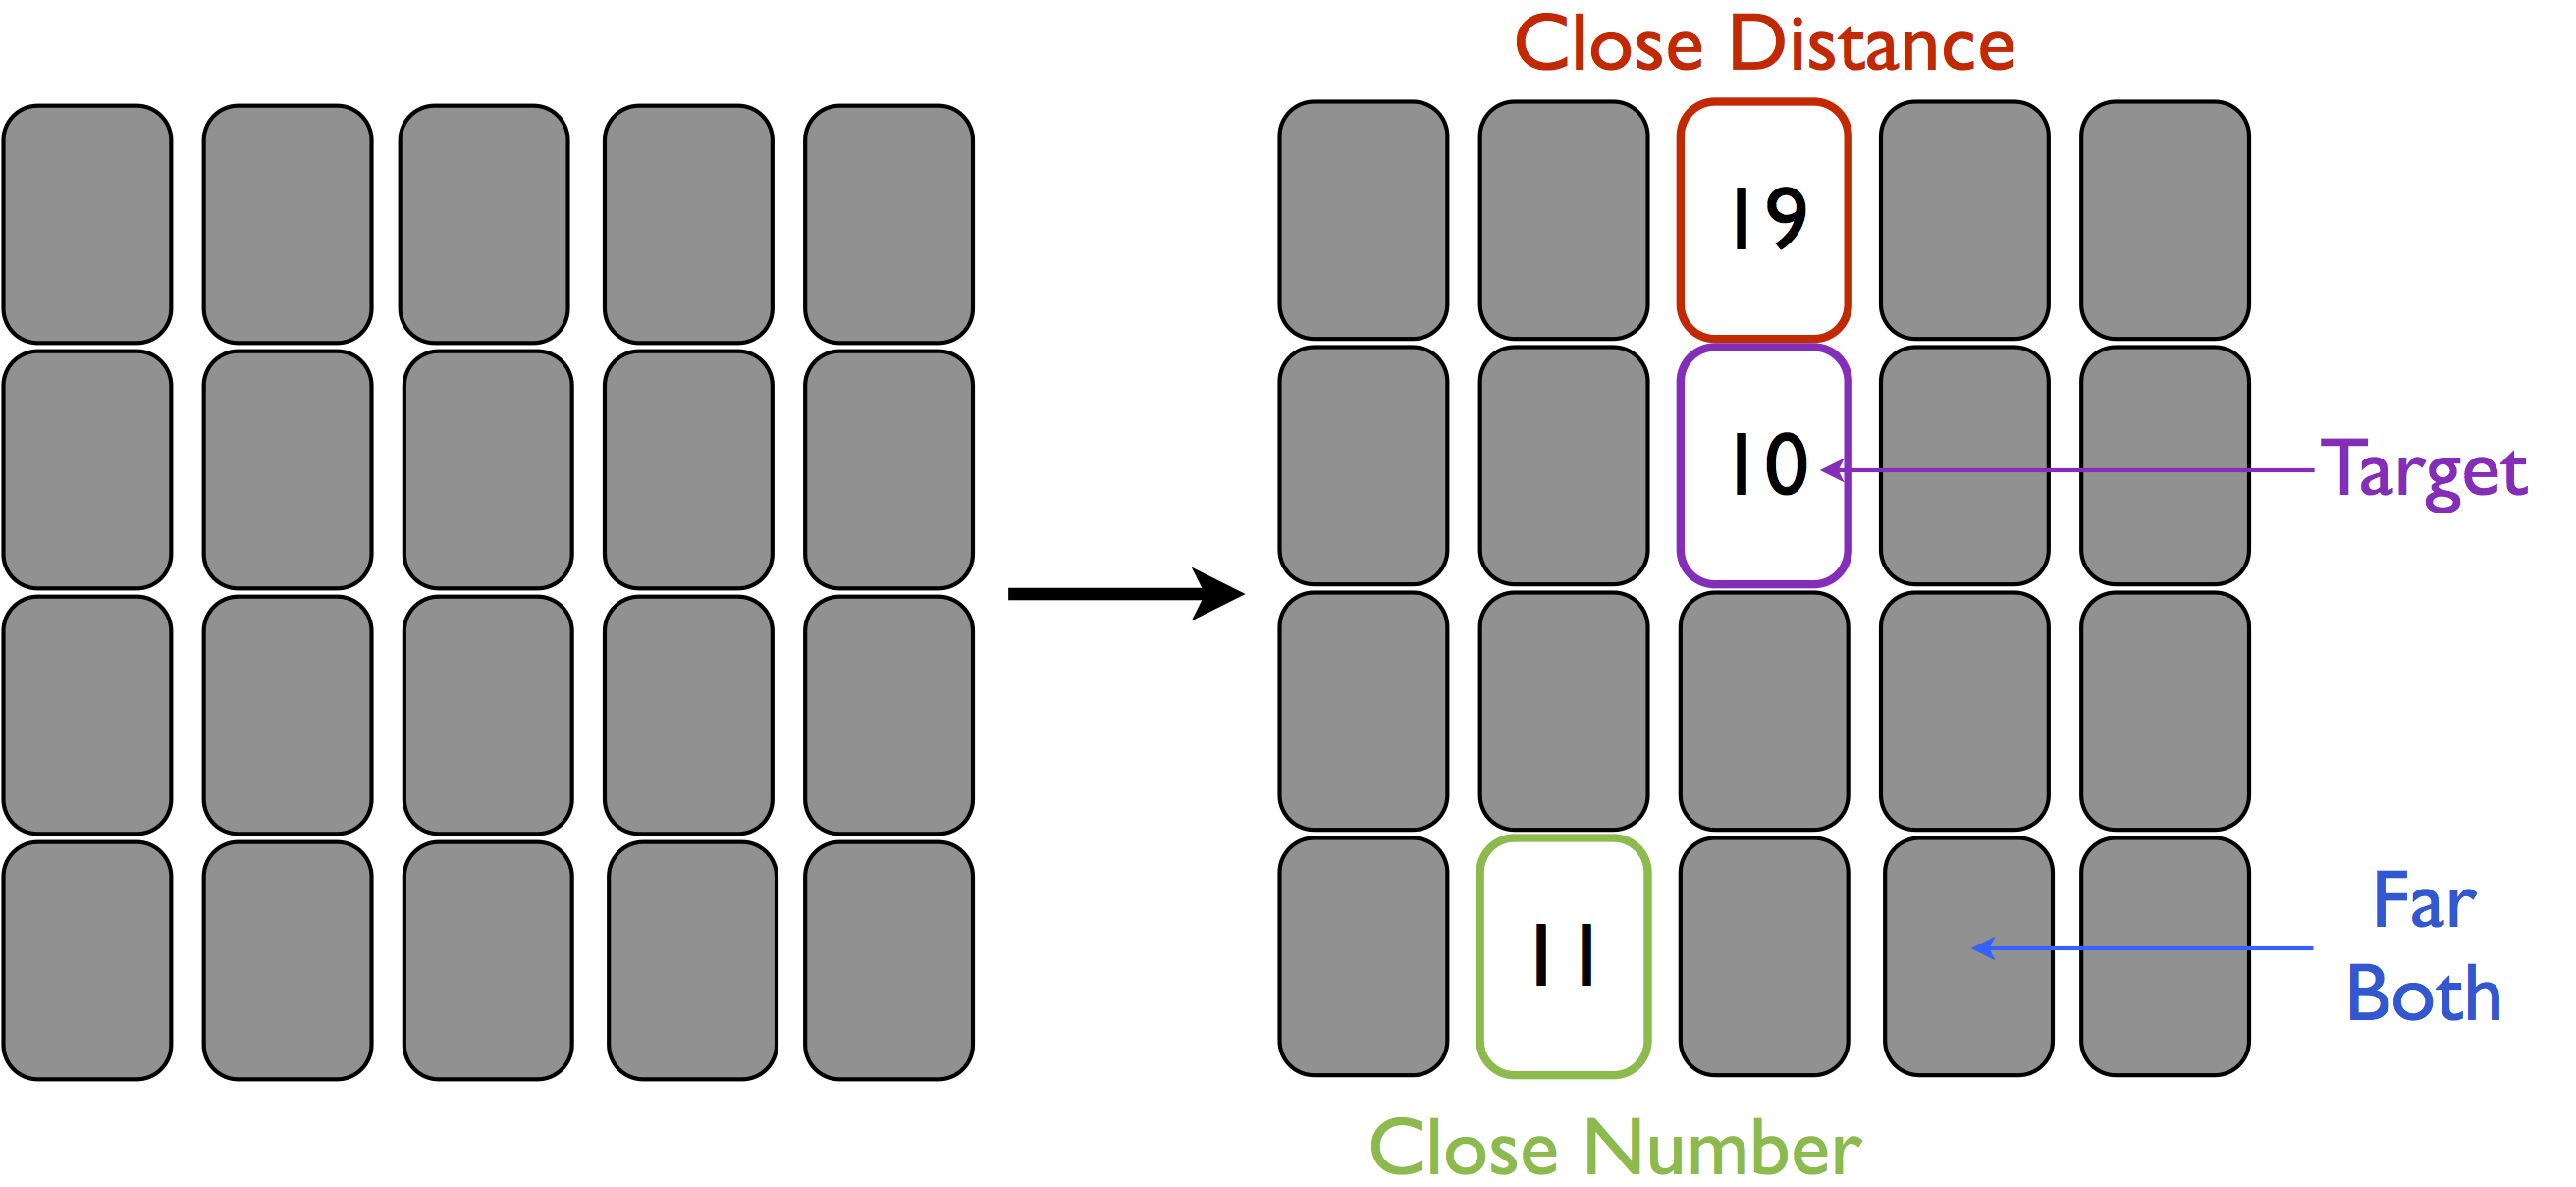
\includegraphics[width=\columnwidth]{images/card_paradigm.png}
\caption{ Expt 2 Paradigm. The target card, 10, is outlined in purple. 19 (red), is \textbf{Proximal}ly close, 11 (green) is \textbf{Numerical}ly close, while 1 (blue) is \textbf{Far} on both proximity and numerosity. }
\label{Expt2ParadigmFig}
\end{figure}

In the Single-Trial-Position (ST-Pos) condition, participants saw a 5x4 array of cards face down. They were told that two characters were playing a game: the cards were numbered 1-20, and they had to pick the number 10 to win. After the characters picked their cards, the winning number 10 is revealed (see Fig. \ref{Expt2ParadigmFig}) There were three possible characters (of which participants only saw two): Scott, who picked 19 (proximally-close), Frank, who picked 11 (numerically-close), and David, who picked 1 (far). Participants rated the emotions of the two characters they saw, before answering a forced-choice question ``Who felt worse?", with the option to say ``Both felt equally bad." In total there are 3 possible pairings (``Proximal vs. Numerical", ``Proximal vs. Far", and ``Numerical vs. Far"), which are all between subject manipulations. Each participant only saw one trial.

The Two-Trial-Position (TT-Pos) condition was similar to the ST-Pos condition, except that after characters picked their cards but before the winning card is revealed, participants make one set of emotion attributions and one forced-choice on who felt worse. Following this, the winning number 10 is revealed, and then participants make another set of attributions.

In the Single-Trial-Number (ST-Num) condition, we changed the rules of the game. There were 19 blank cards, and a target card (circled in purple). Characters were assigned a blank card and had to guess what the number was behind the target card, writing their answers on their assigned blank card. Thus, in the Position conditions, the number of the goal was known (10) while the position was unknown, characters picked a position and were assigned a number (based on their choice); in this Number condition, the position of the goal was known, but the number was unknown, and characters were assigned a position and picked a number. Importantly, the visual description that participants saw is similar to the Position conditions. Thus, after characters wrote their guesses, the winning number behind the purple card is revealed (to be 10). Participants then attributed emotions to the two characters.



\subsubsection{Predictions.}
We predicted that in the Single-Trial-Position condition, proximity would be judged to be a more relevant dimension of closeness than numerously, and so the proximally-close character would be judged to feel worse than the numerically-close character, although the numerically-close character would, to a lesser extent, be judged to feel worse than the character who chose the numerically and proximally far card. In the Single-Trial-Number condition, on the other hand, proximity is irrelevant, and so we predicted that the numerically close character would be judged to feel the worst, and there would be no difference between the proximally close character and the far character.

The Two-Trial-Position condition has an interesting twist. Prior to finding out the position of the winning card, position is still a more relevant dimension than numerosity, but not knowing the position of the winning card makes it impossible to judge closeness based on proximal distance. Observers should judge based on numerosity. At this point, there would be no difference between the proximally close and the far characters, and we predicted that the numerically close character will be judged to feel the worse of them all (similar to ST-Num). However, after finding out the position of the winning card, proximal closeness becomes much more relevant, and we expect to see the proximally close character being judged the worst (similar to ST-Pos).



\begin{figure}[htb!]
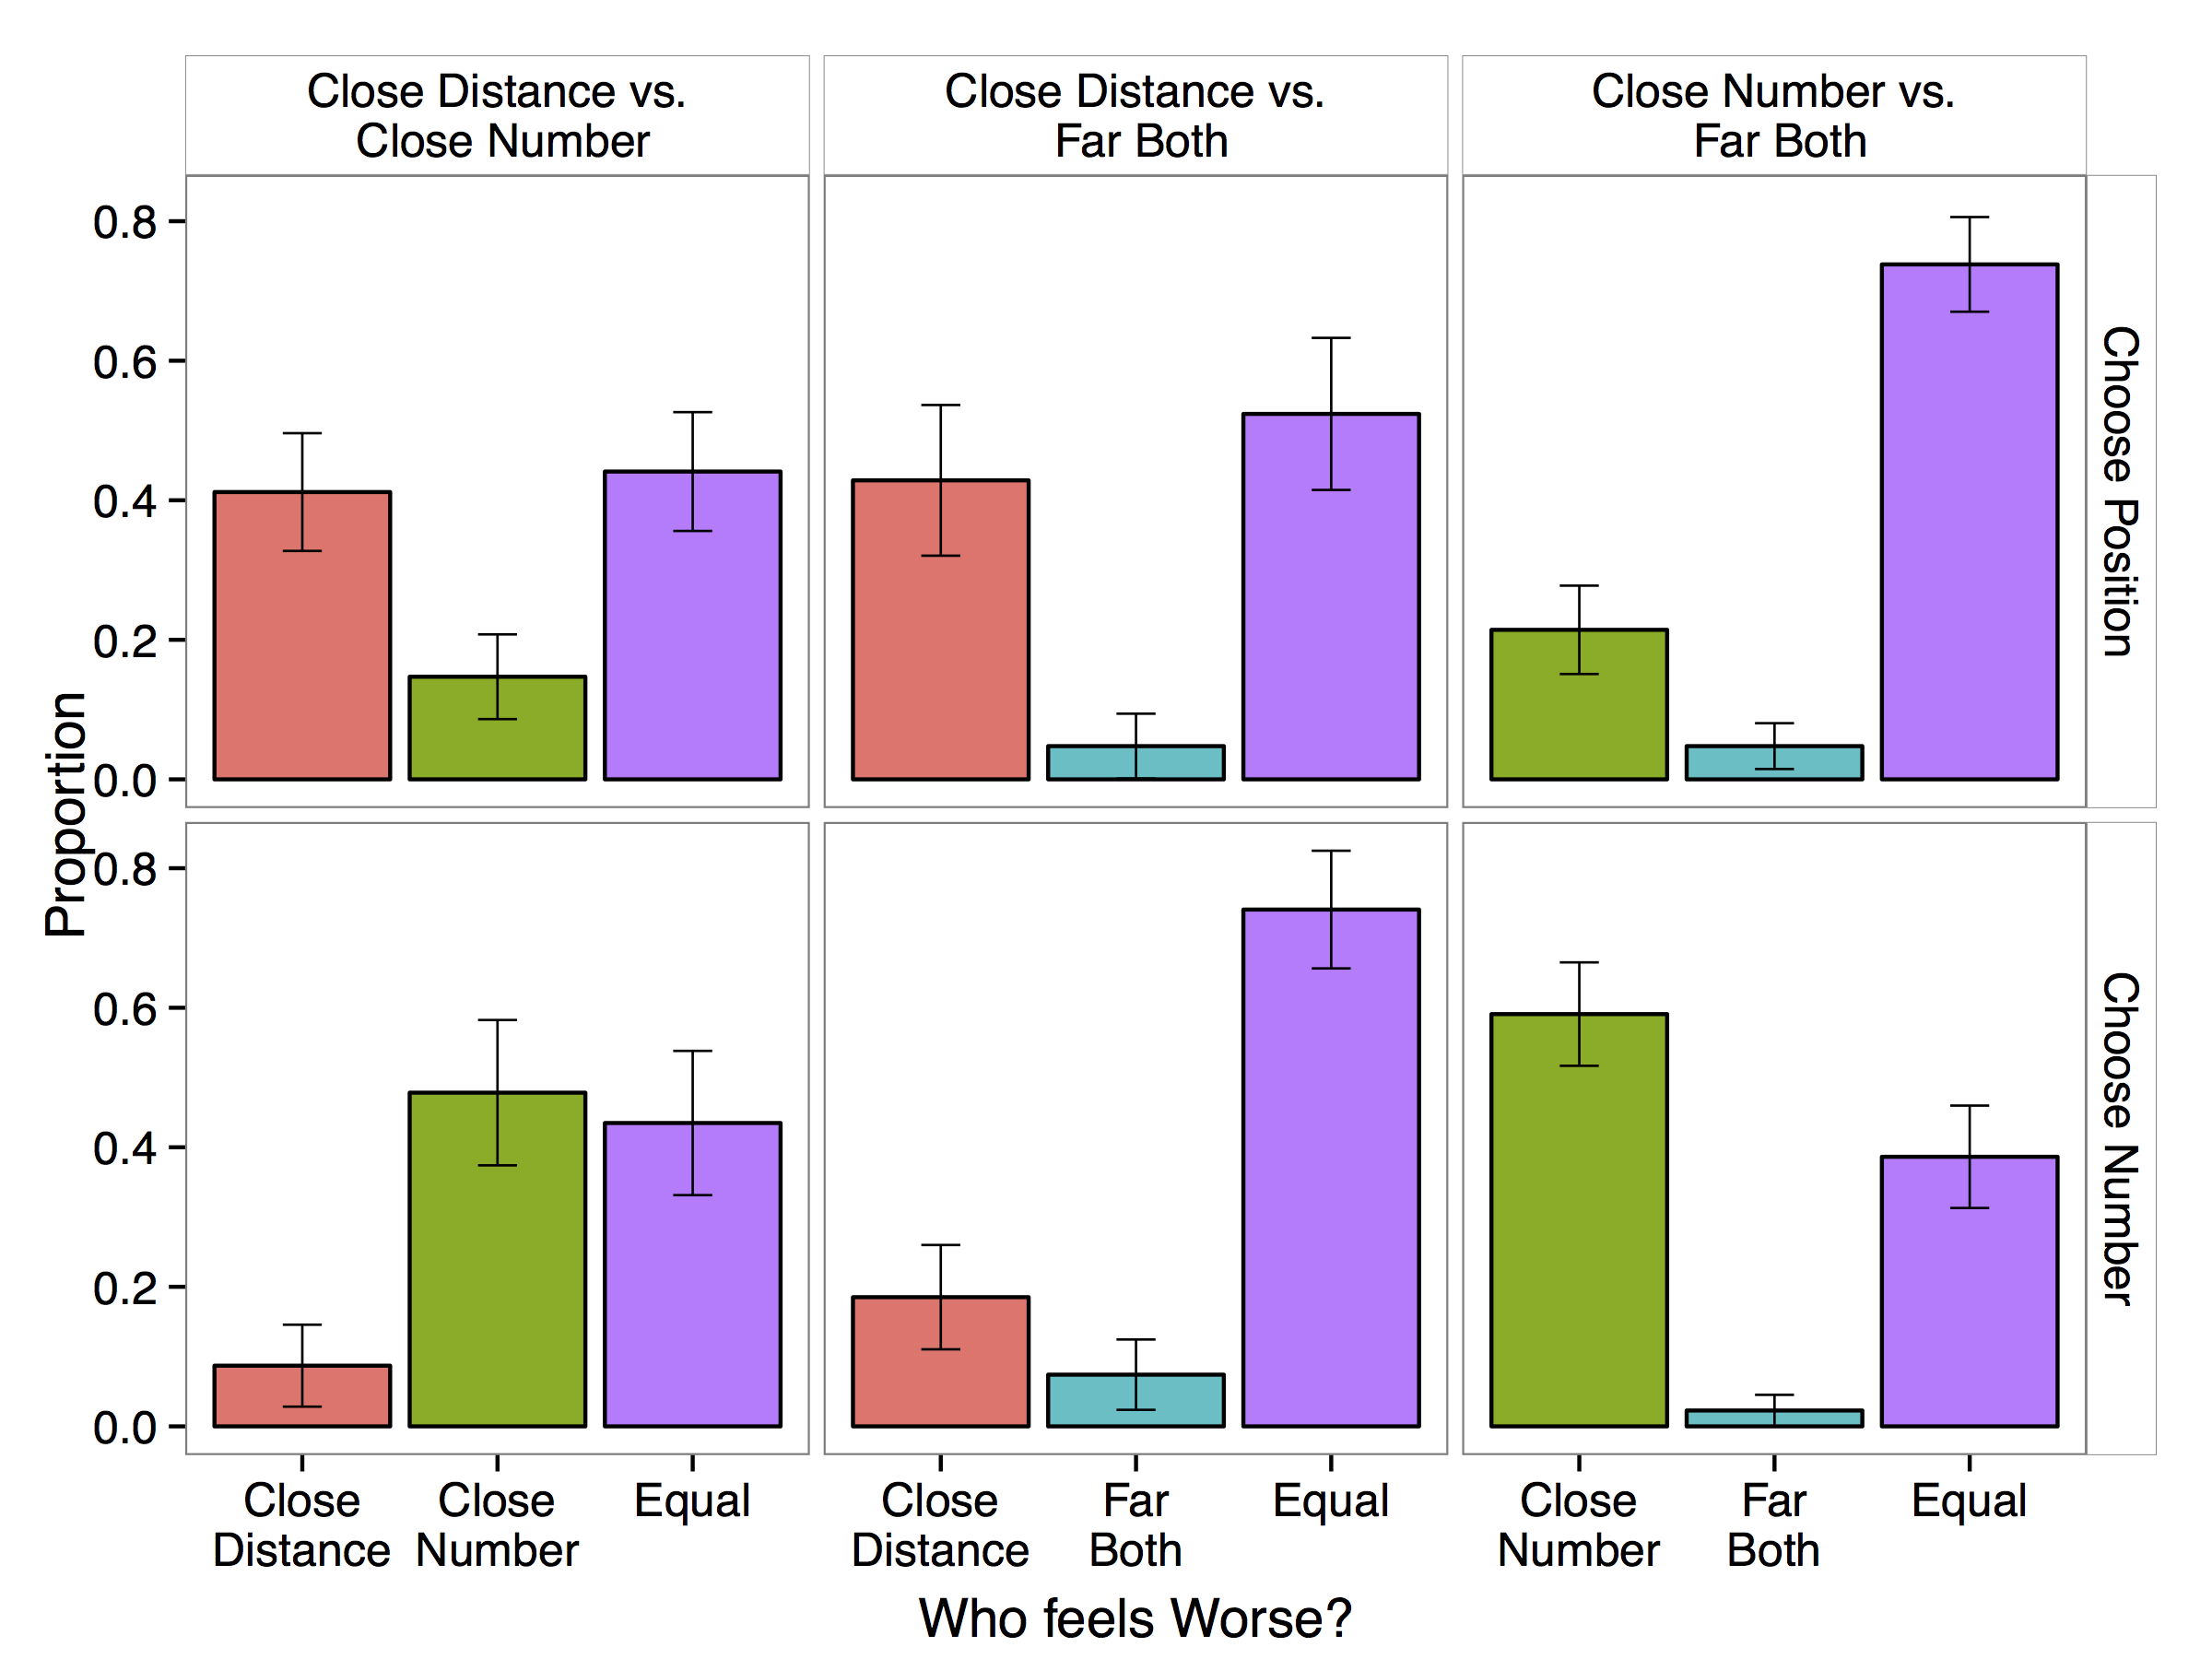
\includegraphics[width=\columnwidth]{images/cardCombined_forcedWorse.png}
\caption{ Expt 2 Results. Proportions of forced choice response. Note that the DV is ``Who feels Worse?" Error bars indicate standard errors. Top row: Single-Trial-Position. 2nd row: Two-Trial-Position, after card is revealed. 3rd row: Two-Trial-Position, before card is revealed. Last row: Single-Trial-Number.}
\label{Expt2ResultFig}
\end{figure}

\subsubsection{Results.}

%%%% TODO XXX STATS

Results for emotion attribution.

The results for the forced-choice ratings are in Fig. \ref{Expt2ResultFig}. In line with our predictions, we find that in the ST-Pos and TT-Pos (after the card was revealed) conditions, the proximally-close character was judged to feel the worst (TODO XXX STATS), and to a much smaller extent, the numerically-close character was judged to feel worse than the far character (TODO XXX STATS). In contrast, in the ST-Num and TT-Pos (before the card was revealed) conditions, the numerically close character is judged to feel worst (TODO XXX STATS).


\section{Experiment 3}
Fitting into model of AffCog

Meta analysis results

\section{Discussion}



%
%In particular, there are 2 main questions that a model should answer:
%How are different types of distances related?
%
%Missing a plane by 5 minutes versus 30 \cite{Kahneman1982}
%
%Missing a goal in soccer by 5 inches versus 30
%
%Entering a store just ahead of a person who won a prize for being the one-millionth customer \cite{Roese1997}
%
%A �near miss� on a slot machine (e.g., Clark, Lawrence, Astley-Jones, \& Gray, 2009)
%
%In a game where one has to roll a 6 on a die to win, rolling a 5 versus rolling a 2 \cite{Kahneman1990}
%
%How do these distances factor (quantitatively) into our affective judgments?
%
%Here, I propose a model of a lay theory of counterfactual distance, a distance measure to the counterfactual world, and in particular, how counterfactual distance might factor into the affective judgments that human observers make about possible counterfactual worlds. These distances---temporal distance; physical distance; semantic distance in some mental representation space; etc---measure the separation between the current world and the counterfactual world being considered. The model proposes how observers consider these other possible worlds and details the affective impact that counterfactual distance has. 



\section{Acknowledgments}

This work was supported in part by an A*STAR National Science Scholarship to DCO and by a James S. McDonnell Foundation Scholar Award to NDG.


\bibliographystyle{apacite}

\setlength{\bibleftmargin}{.125in}
\setlength{\bibindent}{-\bibleftmargin}

\bibliography{cfDistance}


\end{document}
